\subsubsubsubsection{Facility}
\begin{figure}[h]
\centering
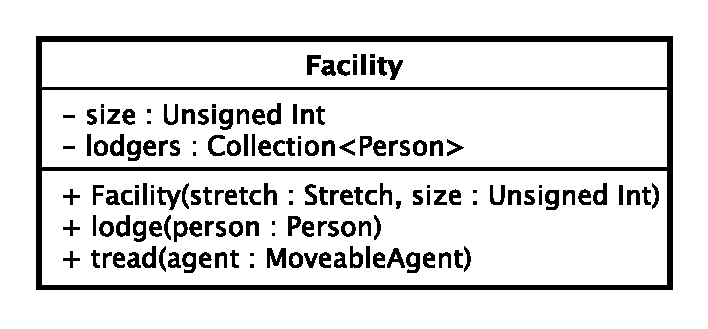
\includegraphics[scale=0.6,keepaspectratio]{images/solution/app/backend/facility.eps}
\caption{\pReactiveComponentStretchDecoration::Facility}
\label{fig:sd-app-facility}
\end{figure}
\FloatBarrier
\begin{itemize}
  \item \textbf{\descr} \\
    It represents a facility which can host several pedestrians.
  \item \textbf{\attrs}
  \begin{itemize}
    \item \texttt{size: Unsigned Int} \\
The maximum number of pedestrians that can be hosted into the facility.
    \item \texttt{lodgers: Collection<Person>} \\
The collection of pedestrians that are currently hosted into the facility.
  \end{itemize}
  \item \textbf{\ops}
  \begin{itemize} 
   \item[+] \texttt{Facility(size: Unsigned Int)} \\
Creates a facility specifying its maximum number of lodgers.
   \item[+] \texttt{lodge(pedestrian: Pedestrian)} \\
If the facility capacity is not full then the pedestrian become a lodger.   
\item[+] \texttt{tread(traveller: Traveller)} \\
Implements the permanence of the agent into the facility. First the facility notifies the traveller that there is a building in the current stretch. After receiving a reply, the facility checks the entities specified in the reply message. If the facility is not full it invokes enter, otherwise the pedestrian is forced to switch to the next step of its route. At the end the facility register itself for a timeout notification.
  \end{itemize}
\end{itemize}
